
\documentclass[12pt,a4paper]{scrartcl}		% KOMA-Klassen benutzen!

\usepackage[utf8]{inputenc}			% Zeichensatzkodierung
\usepackage{graphicx}				% Einbinden von Bildern
\usepackage{color}				% Farben wenn es sein muß
\usepackage{amsmath}		
\usepackage{amsfonts}
\usepackage{listings}

\definecolor{codegreen}{rgb}{0,0.6,0}
\definecolor{codegray}{rgb}{0.5,0.5,0.5}
\definecolor{codepurple}{rgb}{0.58,0,0.82}
\definecolor{backcolour}{rgb}{0.95,0.95,0.95}

\lstdefinestyle{mystyle}{
    backgroundcolor=\color{backcolour},   
    commentstyle=\color{codegreen},
    keywordstyle=\color{magenta},
    numberstyle=\tiny\color{codegray},
    stringstyle=\color{codepurple},
    basicstyle=\ttfamily\footnotesize,
    breakatwhitespace=false,         
    breaklines=true,                 
    captionpos=b,                    
    keepspaces=true,                 
    numbers=left,                    
    numbersep=5pt,                  
    showspaces=false,                
    showstringspaces=false,
    showtabs=false,                  
    tabsize=2
}

\lstset{style=mystyle}

\newcommand\svthema{INF264 Project 1}
\newcommand\svperson{Sophie Blum and Benjamin Friedl}
\newcommand\svdatum{18.09.2020}
\newcommand\lvname{Implementing decision trees}
\begin{document}

\title{ \svthema}
\author{\textsc{\lvname}}
\date{ \small \textsl{\svperson} --- \svdatum }
\maketitle

\abstract
About the document:
The names behind every title point out, who initially wrote the code for this functionality. 

\section{Preprocessing(Sophie)}
\subsection{Visualization}
To get a first idea of the distribution of the datapoints, we visualize them all together in the same graph (figure \ref{fig::all})
This graph gives a first idea of the curvature of the graph, but there are too many datapoints to see patterns directly.
\begin{figure}[h]
    \centering
    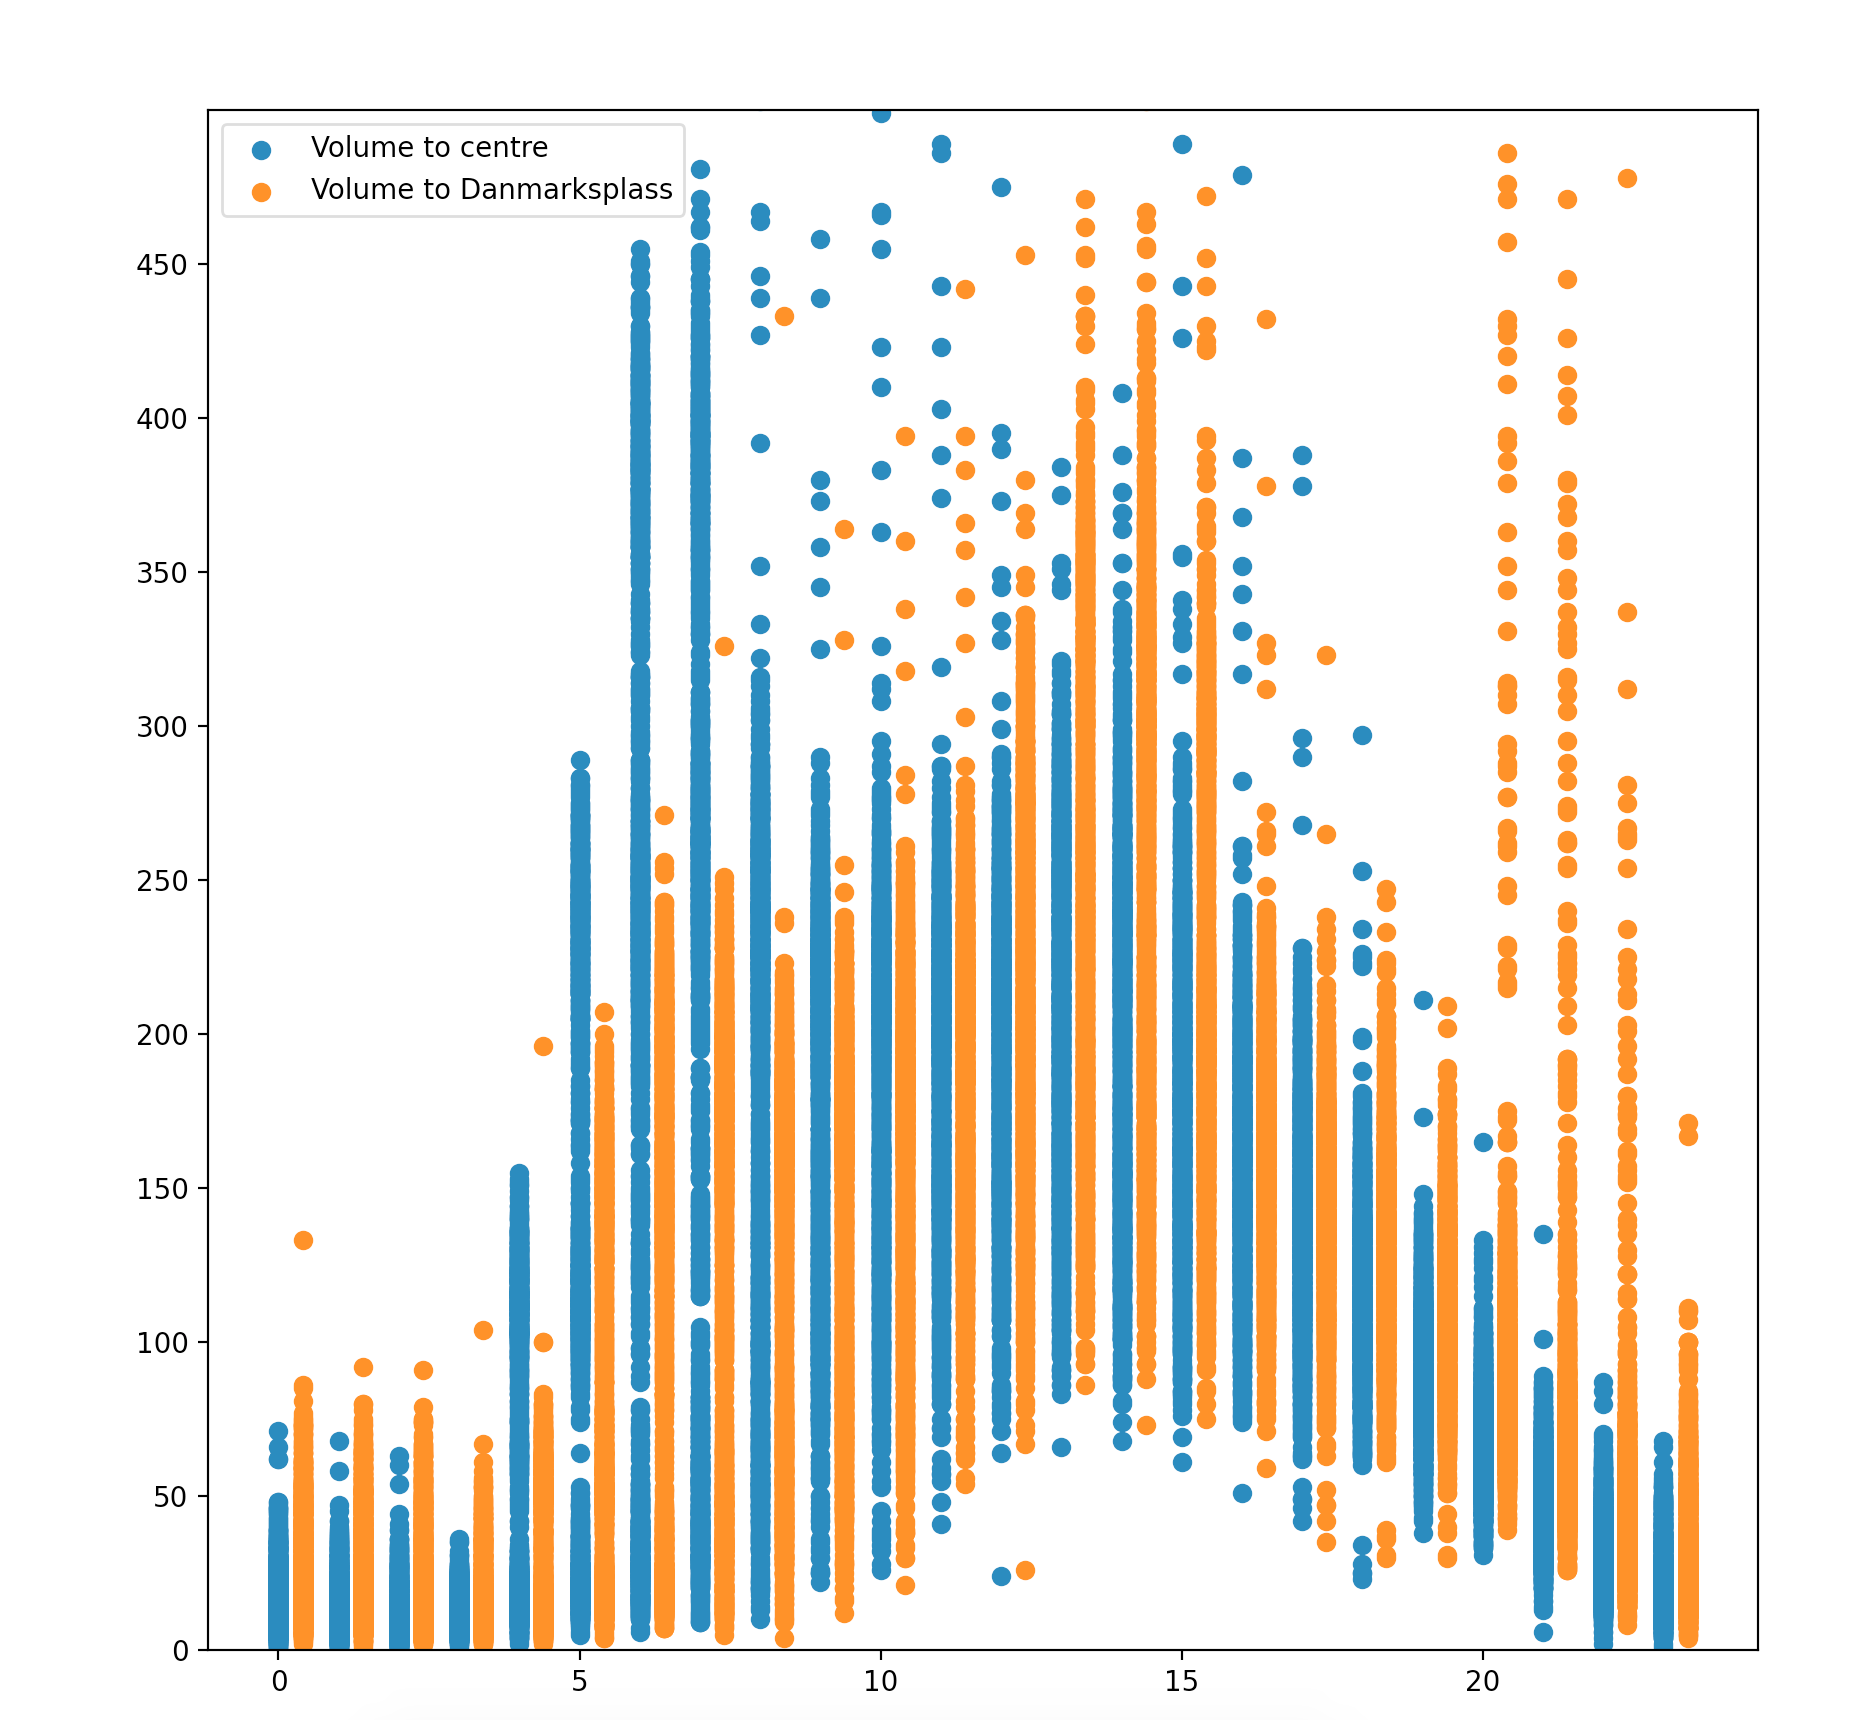
\includegraphics[scale = 0.45]{vis_all.png}
    \caption{All datapoints in one graph}
    \label{fig::all}
\end{figure}

We assume that the traffic volume varies for every weekday or at least from weekdays to sundays. To confirm our assumption, we seperate 
the datapoints according to their weekdays. To achieve that we use datetime objects for each datapoint and the \texttt{weekday()} function.
We also visualize the two directions in seperate colours to compare them in the same diagram (figure \ref{fig::days}).
We do the same visualization for each month, to compare different seasons with each other.
The sorting of the datapoints is summarized in one loop.
\begin{lstlisting}[language=Python]
    dates = []
    weekdays = [[], [], [], [], [], [], []]
    months = [[], [], [], [], [], [], [], [], [], [], [], []]
    for datapoint in X_raw:
        datetime_point = datetime.datetime(datapoint[0], datapoint[1], datapoint[2], hour = datapoint[3])
        new_datapoint = [datetime_point, datapoint[4], datapoint[5], datapoint[6]]
        dates.append(new_datapoint)
        day_indeX_raw = datetime_point.weekday()
        weekdays[day_indeX_raw].append(new_datapoint)
        months[datetime_point.month - 1].append(new_datapoint)
\end{lstlisting}

\begin{figure}[h]
    \centering
    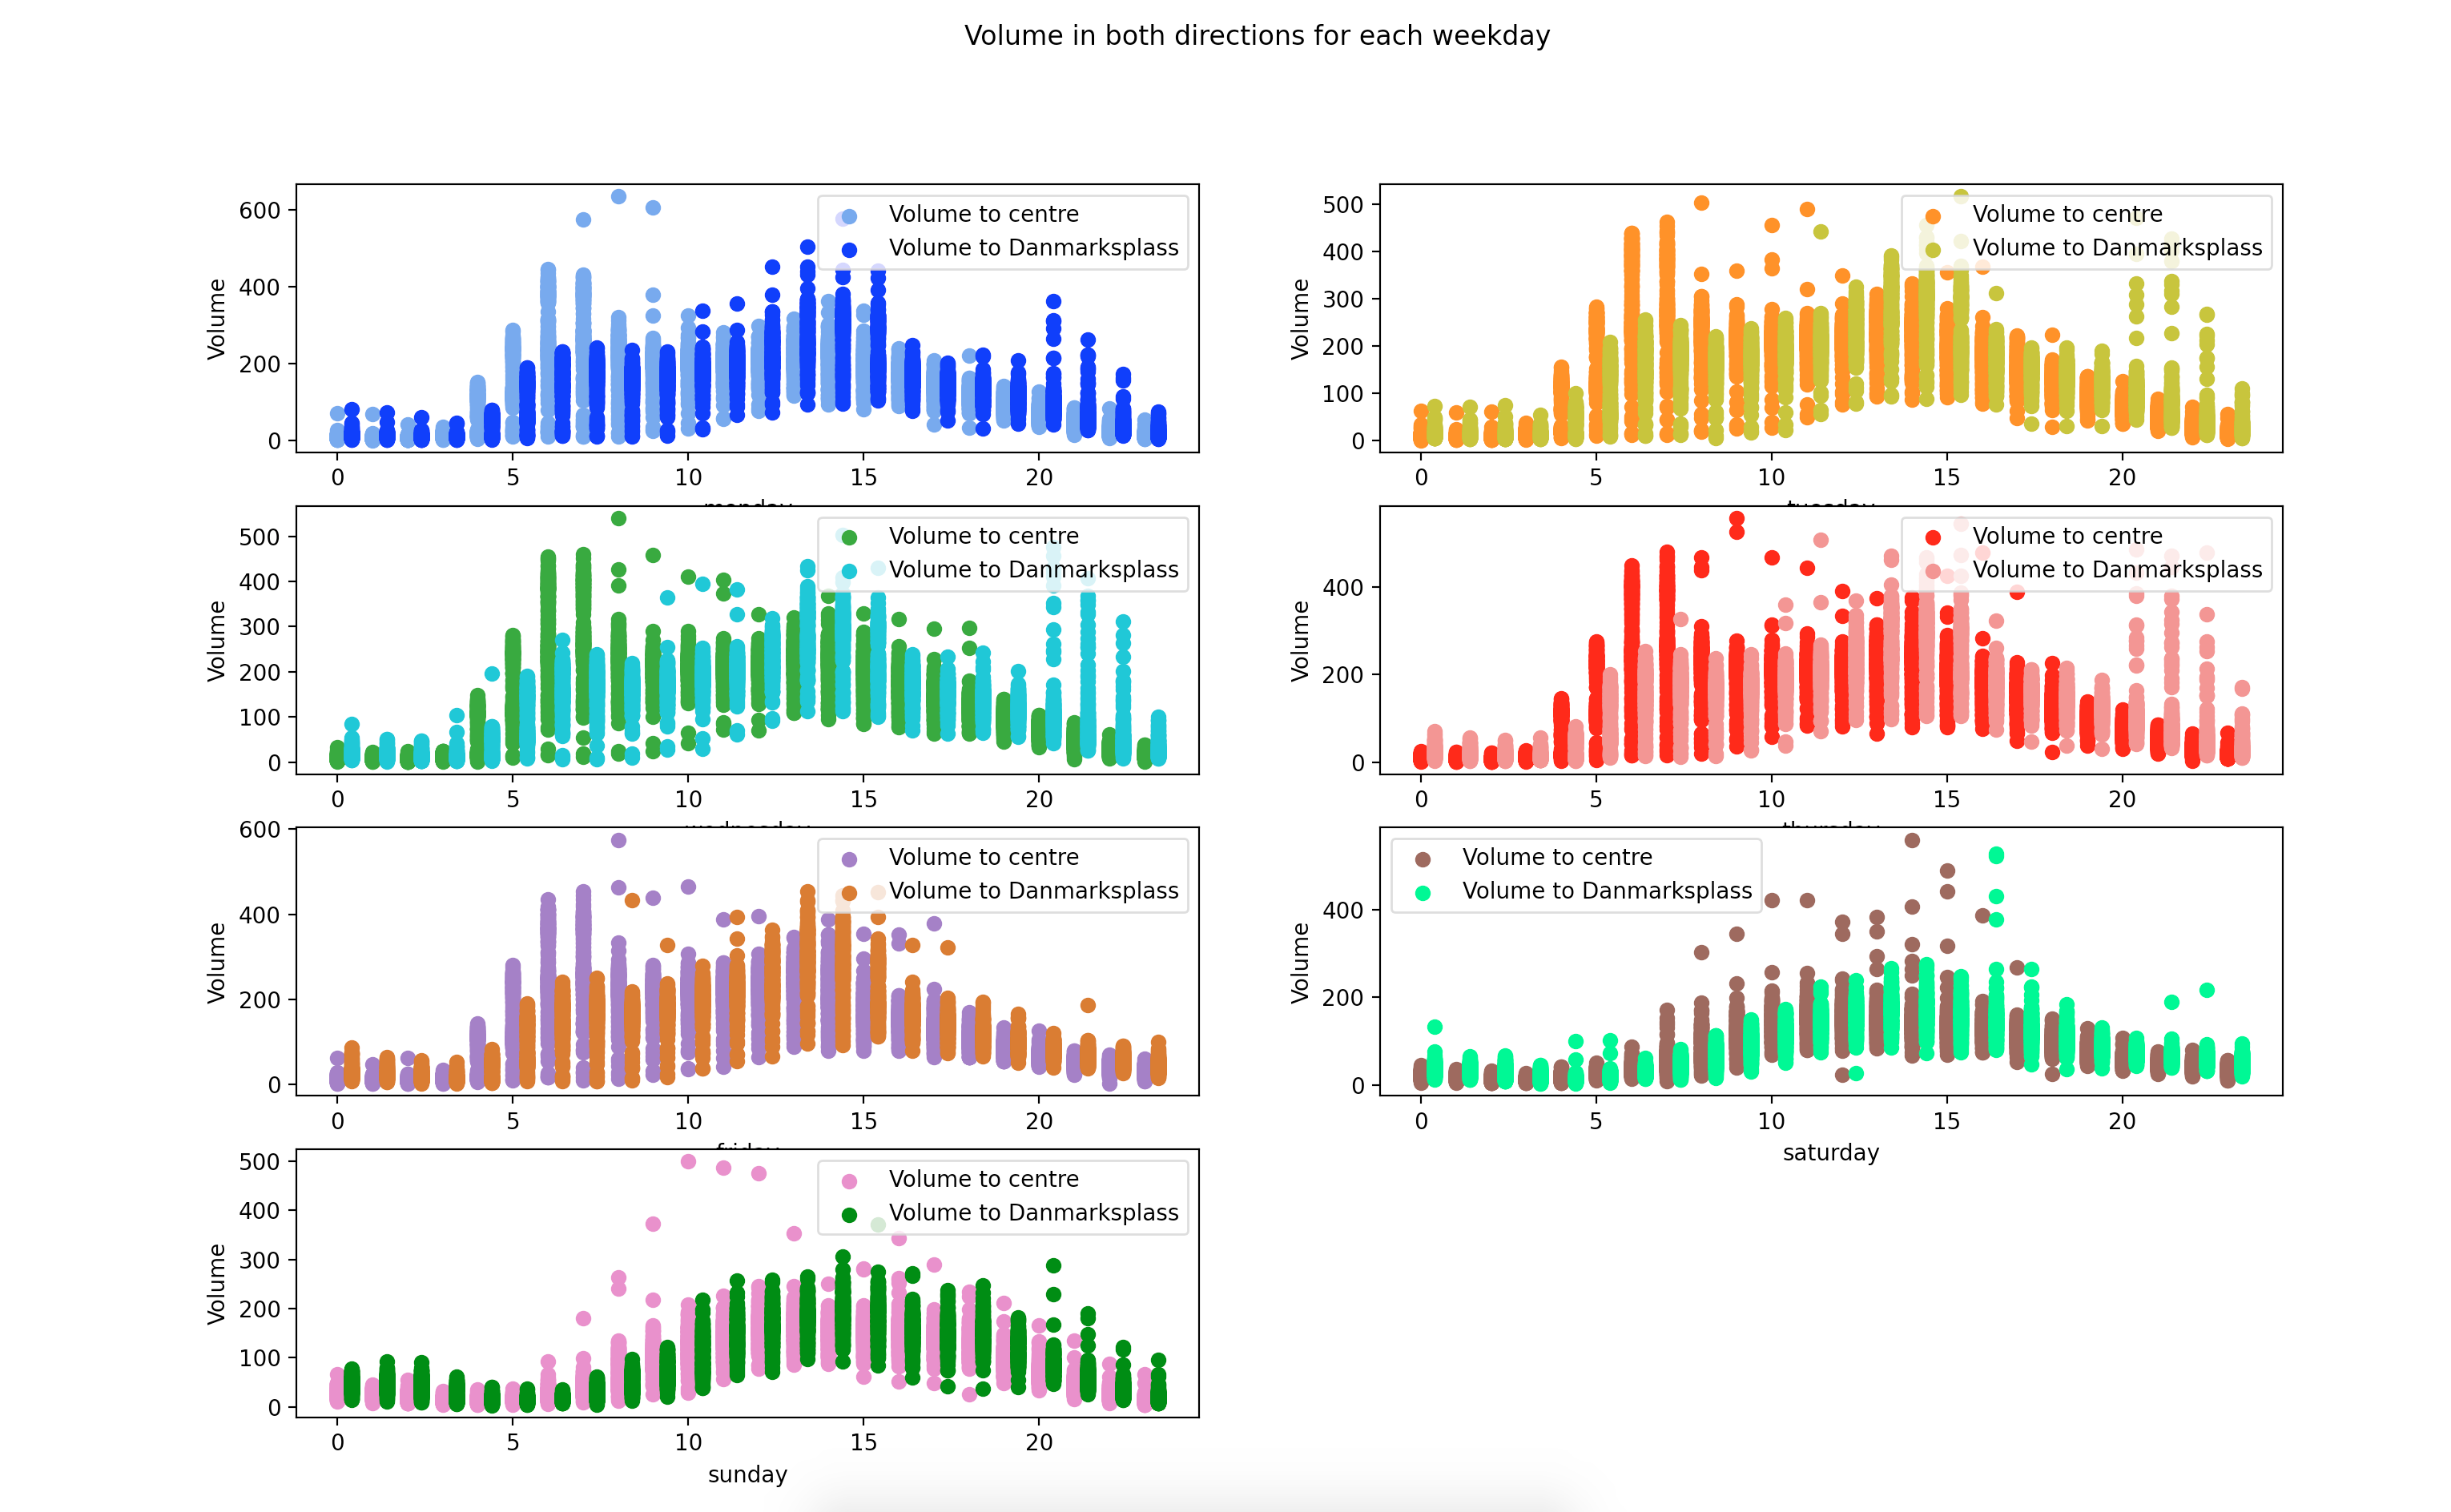
\includegraphics[scale = 0.29]{vis_days.png}
    \caption{Datapoints sorted by weekday}
    \label{fig::days}
\end{figure}

\begin{figure}[h]
    \centering
    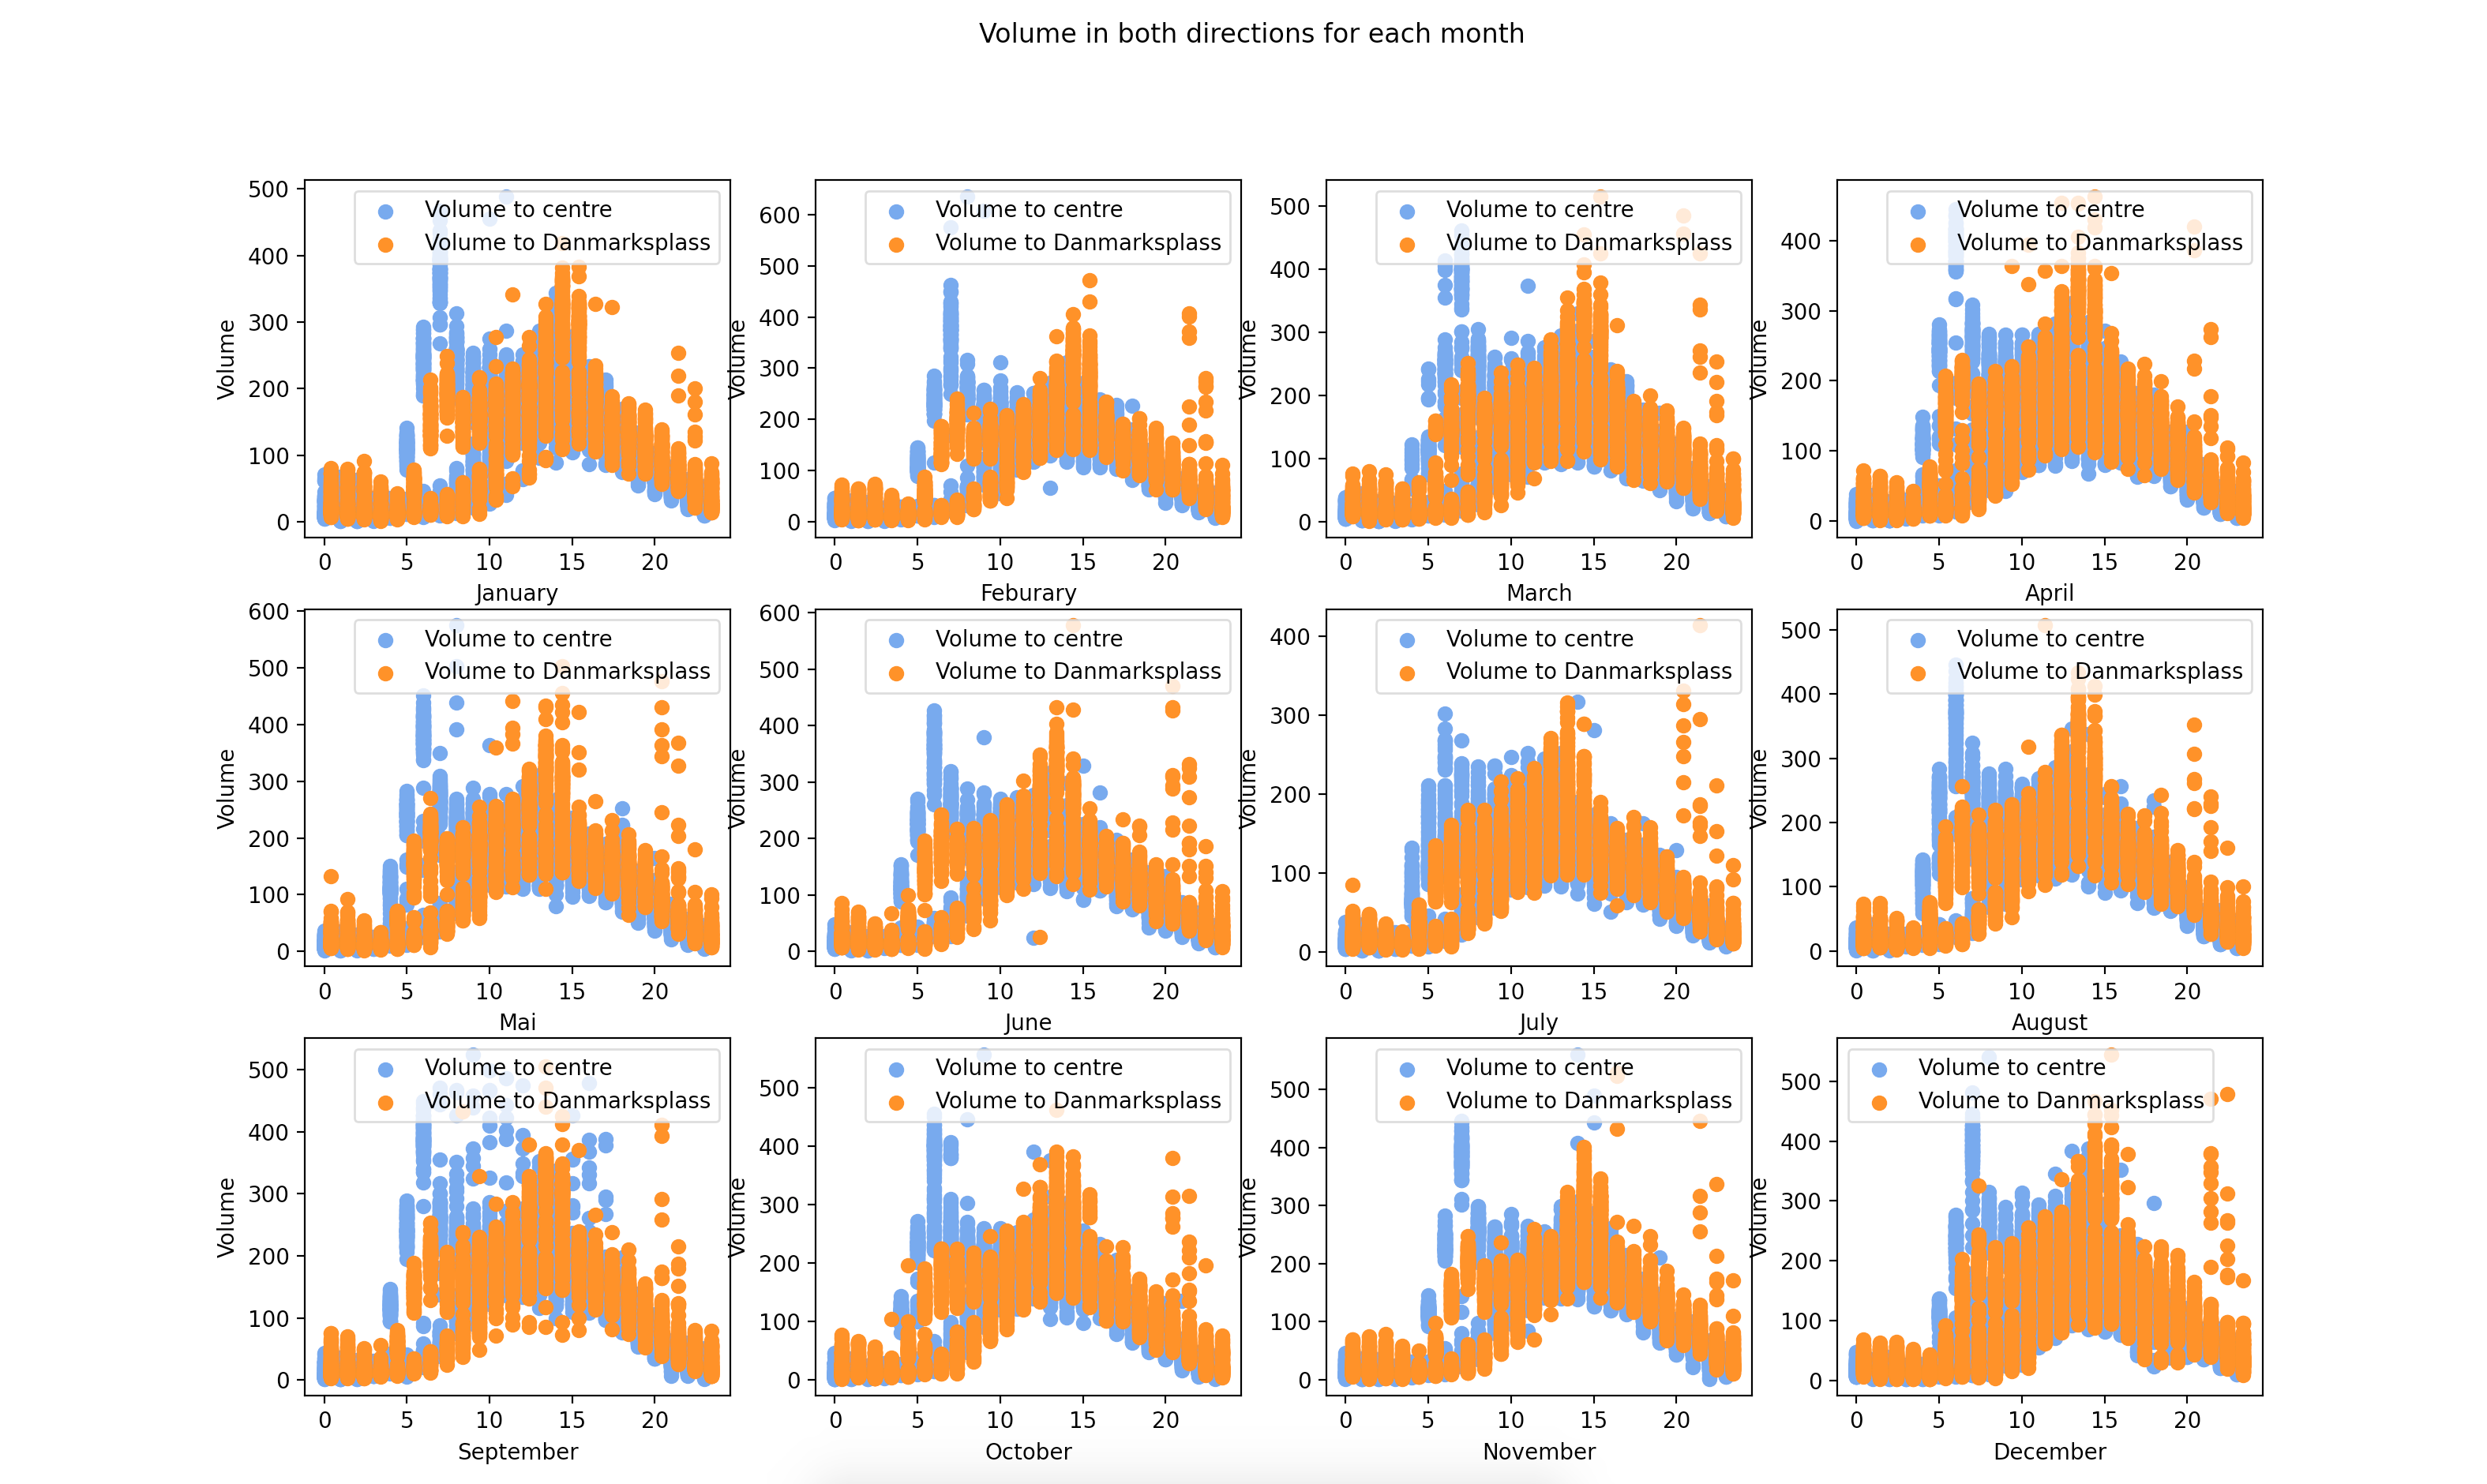
\includegraphics[scale = 0.28]{vis_months.png}
    \caption{Datapoints sorted by month}
    \label{fig::month}
\end{figure}

\subsection{Feature engineering}
Looking closer figure \ref{fig::days}, there are a few observations to make. 
The patterns differ indeed from weekdays to sundays, but saturdays have a pattern of their own as well.
There seems to be more traffic around the afternoon time (likeley the after work rush hour) out of the city centre 
and in the morning into the city centre. At night there is a lot less traffic overall.
The differences between the two directions are most visible during the rush hour times. 
The day could be seperated into daytime blocks to get simpler features, but we decide against that. 
Our reason for that is, that the overall pattern is divisible into blocks, but every hour still has a significant
difference to its neighbouring hours, so we decided to treat the hours of the day as continuous features.
Having a continuous feature for every single date at the same time is not very useful. As we can already see in this 
diagram, the biggest difference is between different weekdays. 
Instead of having the dates as features, we sort the datapoints according to their weekdays and make one-hot-encoding 
features out of it. Every date belongs to one of the three categories: weekday, saturday, sunday/holiday.
As holidays are similar to sundays cocnerning traffic (because there is no rush hour), we take the effort to sort out 
all the holidays as well and declare them as sundays.

To verify our feature choice as it is, we also look at the differences between each month (figure \ref{fig::month}).
We suspect a difference between the seasons, especially winter and summer as there may be less people driving with a car 
in the summer time and rather taking a bike. Looking at the diagram we can't spot significant differences, so we decide 
to not use the season of a given date as an additional feature.

\section{Models}
\subsection{Splitting data}
We used the method “train\_test\_split” to split our data into Training-, Validation and Test-data for all three data-sub-sets 
at the same time to ensure, that we can use the same X\_train for all sub-sets. We chose a ratio of 0.8 for Training-data and 
0.1 for Validation- as well as Test-data to get a good model. 

\begin{lstlisting}[language=Python]
    #Split Data
    seed = 119
    X_train, X_val_test, Y_train_sntr, Y_val_test_sntr, 
    Y_train_dnp, Y_val_test_dnp, Y_train_total, 
    Y_val_test_total
    = model_selection.train_test_split(
        X, Y_sntr, Y_dnp, Y_totalt, test_size= 0.2, 
        shuffle=True, random_state = seed)

    seed = 632
    X_val, X_test, Y_val_sntr, Y_test_sntr, Y_val_dnp, 
    Y_test_dnp, Y_val_total, Y_test_total 
    = model_selection.train_test_split(
        X_val_test, Y_val_test_sntr, Y_val_test_dnp, 
        Y_val_test_total, test_size= 0.5, shuffle=True,
        random_state = seed)
\end{lstlisting}

To use the same code of the models for all data-subsets, we used a for-loop around the model-implementations and renamed the 
currently used data-subset into Y\_train, Y\_val and Y\_test.

\begin{lstlisting}[language=Python]
    different_predictions = ["sentr", "dnp", "total"]
    for p in different_predictions:
        if p == "sntr":
            Y_train = Y_train_sntr
            Y_val = Y_val_sntr
        elif p == "dnp":
            Y_train = Y_train_dnp
            Y_val = Y_val_dnp
        else:
            Y_train = Y_train_total
            Y_val = Y_val_total
    ...
\end{lstlisting}

\subsection{Check function}
We implemented a check-function as “check-stupid-prediction” to use it on all predictions of our models. It gets an array of 
predicted values and returns the amount of predictions that have a value less than zero and is implemented in a simple for-loop.

\begin{lstlisting}[language=Python]
    def check_stupid_prediction(Y):
        count = 0
        for i in range(len(Y)):
            if Y[i] < 0:
                count += 1
        return count
\end{lstlisting}

\subsection{Linear regression with polynomial basic functions}
To build this model, we used a pipeline first transforming the incoming features into polynomial ones and then applying a linear 
regression. For the feature-transformation we used “PolynomialFeatures” from “sklearn.preprocessing”.

\begin{lstlisting}[language=Python]
    for k in klist:
        poly_model = make_pipeline(PolynomialFeatures(k),LinearRegression())
\end{lstlisting}

Using this model, we fit the model using X\_train and Y\_train and let this model predict on our Training- and Validation-data. 
Having this, we calculated the mean-squared-error and r2-score for each polynomial degree in range(1,15) and plotted it to 
search for the best value. 

\begin{lstlisting}[language=Python]
    poly_model.fit(X_train, Y_train)

    Y_train_pred = poly_model.predict(X_train)
    Y_val_pred = poly_model.predict(X_val)
\end{lstlisting}

\subsection{Multiple layer perceptron - regressor}
Our second model is a Multiple Layer Perceptron Regressor for which we tested different values of regularization (alpha), 
learning-rate and count of hidden layers. We used the implementation of sklearn.

Remark: We know that there are further options to optimize the solution, but these weren’t captured in the lecture. 
In addition, we know that the tested values for alpha and the learning-rate might not be optimal or not enough in total, 
but we think this might go beyond the level of competence demanded in this course. 

To test on each combination of 	count of hidden layers, alpha and the learning-rate, we implemented the regressor within 
three for-loops. Again, we fit the model using X\_train and Y\_train and let it predict on X\_train and X\_val to calculate 
the mean-squared-error and r2-score. The latter two are stored in a two-dimensional array which is initialized before 
going into the loops. 

\begin{lstlisting}[language=Python]
    for hiddenlayers in [10,100]:
        i=0
        for learning_rate in learningratelist:
            j=0
            for alpha in alphalist:

                mlp_reg = MLPRegressor(hidden_layer_sizes=(hiddenlayers,), learning_rate ="constant",
                learning_rate_init = learning_rate, alpha = alpha)

                mlp_reg.fit(X_train, Y_train)
                Y_train_pred = mlp_reg.predict(X_train)
                Y_val_pred = mlp_reg.predict(X_val)
\end{lstlisting}

We plotted the values for the mean-squared-error and r2-score for the use on training- and validation-data and the different 
amounts of hidden layers using a three-dimensional wireframe plot. 

We implemented the MLPs for alpha in {0.001, 0.01, 0.1} to capture a wide variety and the learning-rate in {0.01, 0.1, 0.2} 
for the same reason. Originally, we also used the value 0.001 for the learning-rate, but it was too slow in converging. 
For the number of hidden layers, we chose 10 and 100. 

\subsection{KNN-regressor}
Our third model is the K-NN Regressor for which we also used the implementation of sklearn. Similar to the linear regression 
with polynomial basic functions, we built the Regressor for different values of k and calculated the mean-squared-error and 
r2-score on training- as well as validation-data to plot the results and choose a good model. We used k in range(1,15). 

\begin{lstlisting}[language=Python]
    for k in klist:
        knn = KNeighborsRegressor(n_neighbors = k, p=2)
        knn.fit(X_train, Y_train)
        Y_train_pred = knn.predict(X_train)
        Y_val_pred = knn.predict(X_val)
\end{lstlisting}

\section{Results for predicting on training- and validation-data}
\subsection{Predicting towards Sentrum}

\subsubsection{Linear regression with polynomial basic functions}
The minimal mean-squared-error and maximal r2-score is found for k=12 (figure \ref{fig::linregstr}), although it doesn’t change significantly for k in {10,11,12}. 
As the amount of stupid predictions is the same for all values of k in {10,11,12} and is generally amongst the lowest for all k, 
the best of these models is the one for k = 12. The amount of stupid predictions is with 789 on the training-data and 113 on 
validation-data still relatively high in comparison to other models.

\begin{figure}[h]
    \centering
    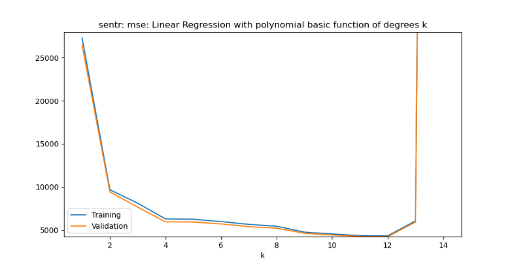
\includegraphics[scale = 0.8]{sntr_linreg_mse.png}
    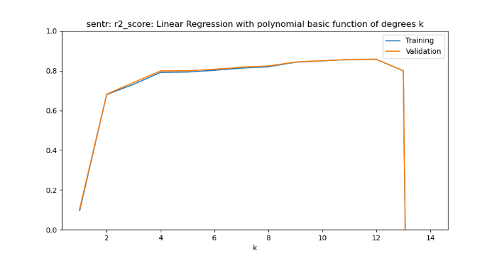
\includegraphics[scale = 0.8]{sntr_linreg_r2.png}
    \caption{Linear regression error sentrum}
    \label{fig::linregstr}
\end{figure}

\subsubsection{MLP-regressor}
\subparagraph{With 10 hidden layers}
one can see that there seem to be a lot of local maxima and minima in the mean-squared-error and r2-score (figure \ref{fig::mlpstr10}). The lowest value for the 
mean-squared-error on validation-data is reached for the learningrate = 0.1 and alpha = 0.01. The amount of stupid predictions for this model is 0.
\begin{figure}[h]
    \centering
    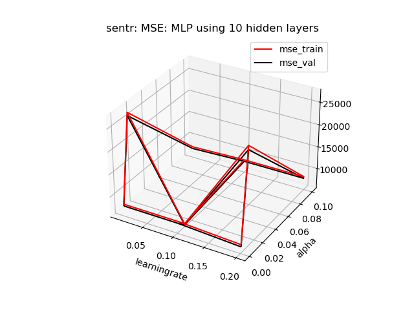
\includegraphics[scale = 1]{sntr_mlp_mse_10.png}
    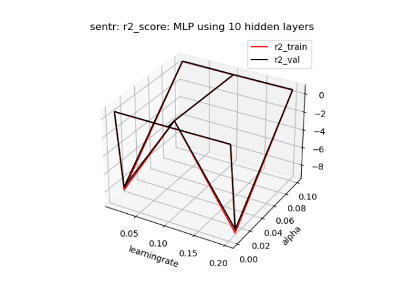
\includegraphics[scale = 1]{sntr_mlp_r2_10.png}
    \caption{MLP 10 hidden layers error sentrum}
    \label{fig::mlpstr10}
\end{figure}

\subparagraph{With 100 hidden layers}
there seem to be a lot of local minima and maxima again which can’t be captured for only three values for alpha and the learning-rate (figure \ref{fig::mlpstr100}). 
Generally, the error is lower than with using 10 hidden layers. The lowest value for the mean-squared-error is achieved for learningrate = 0.01 and alpha = 0.1 with 4335. 
The higher value of alpha is not surprising as without regularization this model easily overfits. For all values of alpha and the learning-rate the number of stupid 
predictions is 0.

\begin{figure}[h]
    \centering
    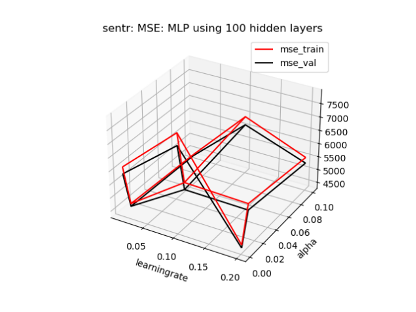
\includegraphics[scale = 1.1]{sntr_mlp_mse_100.png}
    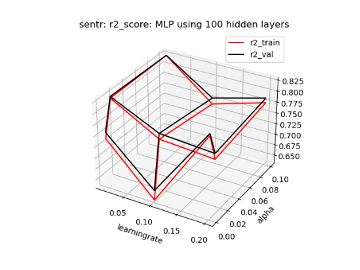
\includegraphics[scale = 1.1]{sntr_mlp_r2_100.png}
    \caption{MLP 100 hidden layers error sentrum}
    \label{fig::mlpstr100}
\end{figure}

\subsubsection{KNN-regressor}
These models make the best predictions for k=12 with a mean-squared-error of 4270 on the validation-data, although it starts stagnating at k=10 (figure \ref{fig::knnstr}). 
The number of stupid predictions is 0 for every k, as all values in Y\_train are greater than 0. The high error for k=1 is only explainable for us through the heuristic 
search for neighbours.\\

\begin{figure}[h]
    \centering
    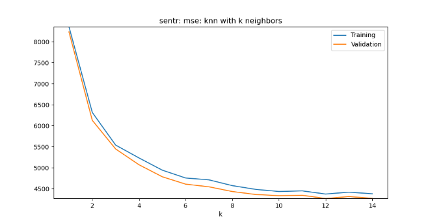
\includegraphics[scale = 0.8]{sntr_knn_mse.png}
    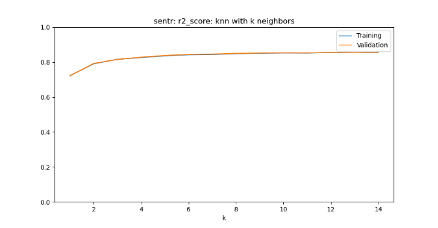
\includegraphics[scale = 0.8]{sntr_knn_r2.png}
    \caption{KNN error sentrum}
    \label{fig::knnstr}
\end{figure}

Generally, the lowest validation-error is reached for the K-NN with k=12, although it isn’t significantly lower as for the MLP with 100 hidden layers. 
Because the K-NN needs a lot more memory and time for predicting we chose the MLP with 100 hidden layers, learning-rate=0.01 and alpha=0.1. 

\subsection{Predicting towards Danmarksplass}

\subsubsection{Linear regression with polynomial basic functions}
The polynomial models make the best predictions for k = 12 with a mean-squared-error of 1212 on  validation-data (figure \ref{fig::linregdnp}). 
The number of stupid predictions is 0. 

\begin{figure}[h]
    \centering
    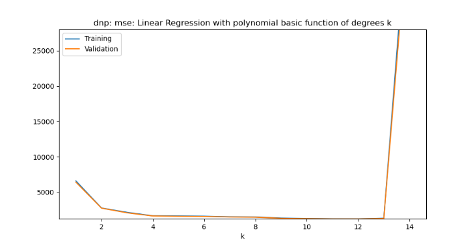
\includegraphics[scale = 0.8]{dnp_linreg_mse.png}
    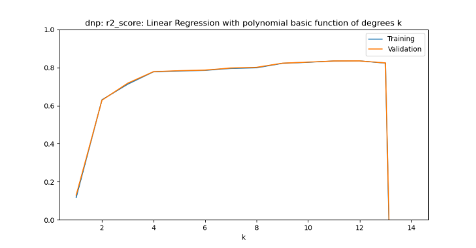
\includegraphics[scale = 0.8]{dnp_linreg_r2.png}
    \caption{Linear regression error danmarksplass}
    \label{fig::linregdnp}
\end{figure}

\subsubsection{MLP-regressor}
\subparagraph{With 10 hidden layers}
the models make the best predictions for alpha=0.01 and learningrate=0.01 with a mean-squared-error of 1352, although there are other configurations with almost as 
low values (figure \ref{fig::mlpdnp10}). The amount of stupid predictions is 0 for this configuration. 

\begin{figure}[h]
    \centering
    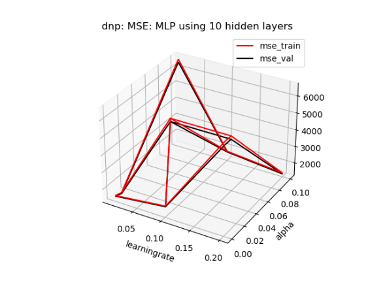
\includegraphics[scale = 1.1]{dnp_mlp_mse_10.png}
    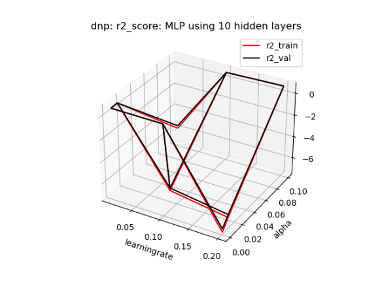
\includegraphics[scale = 1.1]{dnp_mlp_r2_10.png}
    \caption{MLP 10 hidden layers error danmarksplass}
    \label{fig::mlpdnp10}
\end{figure}

\subparagraph{With 100 hidden layers}
the models make the best predictions for alpha=0.1 and learningrate=0.01 with the significantly highest r2-score and the second-best mean-squared-error of 1175
(figure \ref{fig::mlpdnp100}). 
The amount of stupid predictions is 0. 

\begin{figure}[h]
    \centering
    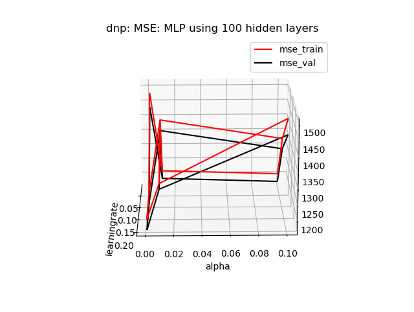
\includegraphics[scale = 1.1]{dnp_mlp_mse_100.png}
    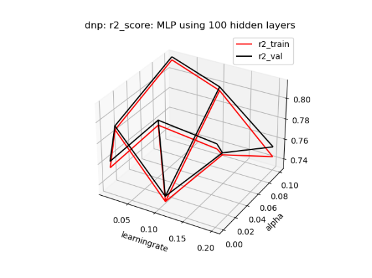
\includegraphics[scale = 1.1]{dnp_mlp_r2_100.png}
    \caption{MLP 100 hidden layers error danmarksplass}
    \label{fig::mlpdnp100}
\end{figure}

\subsubsection{KNN-regressor}
These models make the best predictions for k = 10 with a mean-squared-error of 1248 on validation-data (figure \ref{fig::knndnp}). 
The amount of stupid predictions is again 0 for every k. 

\begin{figure}[h]
    \centering
    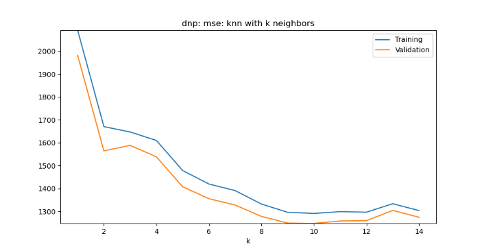
\includegraphics[scale = 0.8]{dnp_knn_mse.png}
    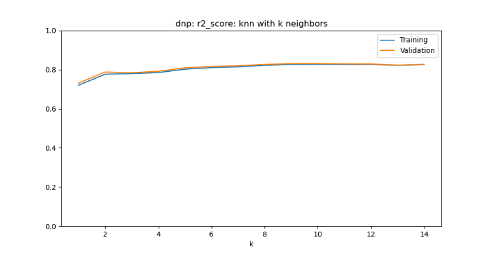
\includegraphics[scale = 0.8]{dnp_knn_r2.png}
    \caption{KNN error danmarksplass}
    \label{fig::knndnp}
\end{figure}

The best predictions of all these models are done by the MLP using 100 hidden-layers, alpha=0.1 and learningrate=0.01.

\subsection{Predicting total amount}

\subsubsection{Linear regression with polynomial basic functions}
These models make the best predictions for k = 12 with a mean-squared-error of 4221 on the validation-data (figure \ref{fig::linregtotal}). 
The amount of stupid predictions is with 789 on training-data and 113 on validation-data amongst the lower ones for this model-family. 

\begin{figure}[h]
    \centering
    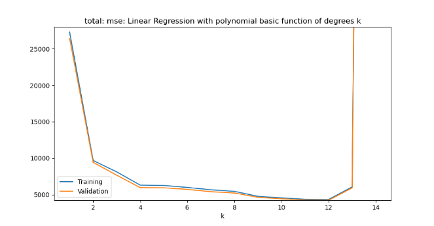
\includegraphics[scale = 0.8]{total_linreg_mse.png}
    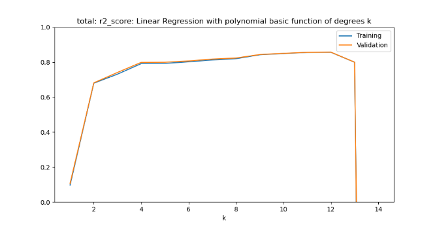
\includegraphics[scale = 0.8]{total_linreg_r2.png}
    \caption{Linear regression error total}
    \label{fig::linregtotal}
\end{figure}

\subsection{MLP-regressor}

\subparagraph{Using 10 hidden layers}
the models make the best predictions for learningrate = 0.01 and alpha = 0.1 with a mean-squared-error of 5656 on the validation-data and 0 stupid predictions
(figure \ref{fig::mlptotal10}). 

\begin{figure}[h]
    \centering
    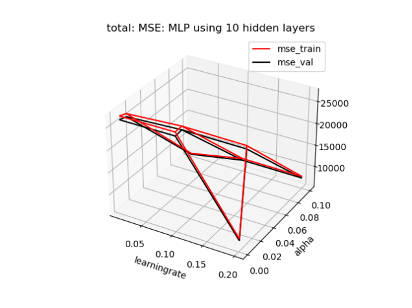
\includegraphics[scale = 1]{total_mlp_mse_10.png}
    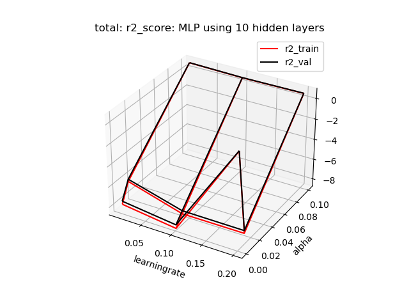
\includegraphics[scale = 1]{total_mlp_r2_10.png}
    \caption{MLP 10 hidden layers error total}
    \label{fig::mlptotal10}
\end{figure}

\subparagraph{Using 100 hidden layers}
the models make the best predictions for learningrate = 0.2 and alpha = 0.1 with a mean-squared-error of 4260 on the validation-data and 0 stupid predictions
(figure \ref{fig::mlptotal100}).

\begin{figure}[h]
    \centering
    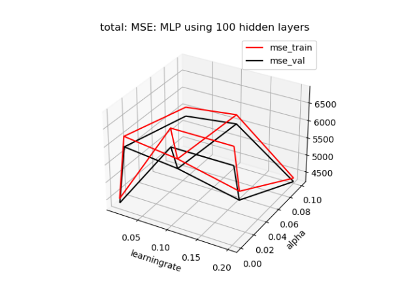
\includegraphics[scale = 1]{total_mlp_mse_100.png}
    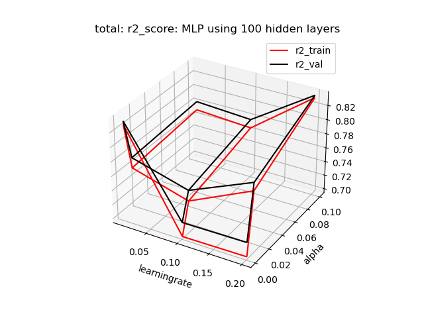
\includegraphics[scale = 1]{total_mlp_r2_100.png}
    \caption{MLP 100 hidden layers error total}
    \label{fig::mlptotal100}
\end{figure}

\subsection{KNN-regressor}
These models make the best predictions for k = 12 with a mean-squared-error of 4270 on the validation-data (figure \ref{fig::knntotal}). 
The number of stupid predictions is again 0 for every k. 

\begin{figure}[h]
    \centering
    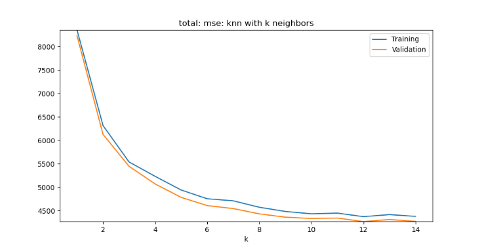
\includegraphics[scale = 0.8]{total_knn_mse.png}
    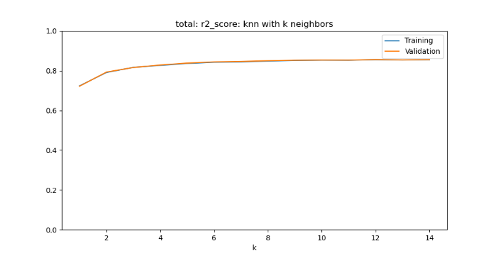
\includegraphics[scale = 0.8]{total_knn_r2.png}
    \caption{KNN error total}
    \label{fig::knntotal}
\end{figure}

The lowest mean-squared-error on validation-data for all these models is reached for the Linear Regression with polynomial basic functions of degree 12. Nevertheless, 
this model makes some stupid prediction and the MLP with 100 hidden layers, learningrate = 0.2 and alpha = 0.1 doesn’t have a significantly higher error. 
Therefore, we chose the latter model for predicting the total amount.

\section{Results on the testing data}
Now the best model for each prediction-task is used on the test data to estimate the error. 

\subsection{Predicting towards Sentrum}
The chosen model was the MLP-Regressor using 100 hidden layers, learningrate=0.01 and alpha=0.1. The mean-squared-error on the testing-data is 1430 and the r2-score 0.8146. 
This is a lot lower than the validation-error of 4335 and therefore doesn’t seem to represent the true error. There are no stupid predictions.
\subsection{Predicting towards Danmarksplass}
The chosen model was also the MLP-Regressor using 100 hidden layers, learningrate=0.01 and alpha=0.1. The mean-squared-error on the testing-data is 1534 and the r2-score is 0.7416. 
This is slightly higher than the error on the validation-data. There are no stupid predictions.
\subsection{Predicting total amount}
The chosen model was an MLP-Regressor using 100 hiddenlayers, learning-rate=0.2 and alpha=0.1. The mean-squared-error on the testing-data is 5094 and the r2-score is 0.81632. 
This is also slightly worse in comparison to the error on validation-data. There are no stupid predictions. 

\section{Evaluation}
\subsection{Comparison of Danmarksplass and Sentrum}
Although we chose the same kind of model for both directions, it is likeley, that the models differ.
The differences in the data points can be seen in figure \ref{fig::days}. As the patterns in the datapoints 
are different, the models trained on them will also be fitted to these patterns.

The models we chose do not make any unrealistic predictions and perform overall well. 
Looking at the datapoints in figure \ref{fig::days} one can see how much the points vary at a given hour (large variance).
As the hours are one of the underlying features, the models are trained on data with variance.
The errors are therefore also slightly bigger.

\subsection{Model performance in 2020}
As already mentioned, we assume the patterns in the data are caused by rush hours during weekdays. These patterns are significantly less accurate in 2020 due to Covid-19.
As a lot of employees worked from home a majority of the year, the rush hour traffic is also less in both directions. Therefore the model would perform less good on the 2020 data.
We can see in this case, that no model can predict unexpected events and their impact on data. We can always only learn patterns and apply the learned patterns to new data.
If these patterns change unexpectedly, our models are not able to predict the new unexpected behaviour.

\end{document}